% ==============================================================================
% Modelo para Especificação de Projeto de Software
% Prof. Vítor E. Silva Souza - NEMO/UFES :: DI/UFES :: PPGI/UFES
%
% Baseado em abtex2-modelo-trabalho-academico.tex, v-1.9.2 laurocesar
% Copyright 2012-2014 by abnTeX2 group at http://abntex2.googlecode.com/ 
%
% This work may be distributed and/or modified under the conditions of the LaTeX 
% Project Public License, either version 1.3 of this license or (at your option) 
% any later version. The latest version of this license is in
% http://www.latex-project.org/lppl.txt.
%
% IMPORTANTE:
% Instruções encontram-se espalhadas pelo documento. Para facilitar sua leitura,
% tais instruções são precedidas por (*) -- utilize a função localizar do seu
% editor para passar por todas elas.
% ==============================================================================

% Usa o estilo abntex2, configurando detalhes de formatação e hifenização.
\documentclass[
	12pt,				
	oneside,		
	a4paper,			
	english,			% Idioma adicional para hifenização.
	french,				% Idioma adicional para hifenização.
	spanish,			% Idioma adicional para hifenização.
	brazil				% O último idioma é o principal do documento.
	]{abntex2}


%%% Importação de pacotes. %%%

% Conserta o erro "No room for a new \count". 
% O comando \reserveinserts deve ser comentado ou não, dependendo da versão do LaTeX.
\usepackage{etex}
%\reserveinserts{28}

% Usa a fonte Latin Modern.
\usepackage{lmodern}

% Seleção de códigos de fonte.
\usepackage[T1]{fontenc}

% Codificação do documento em Unicode.
\usepackage[utf8]{inputenc}

% Usado pela ficha catalográfica.
\usepackage{lastpage}

% Indenta o primeiro parágrafo de cada seção.
\usepackage{indentfirst}

% Controle das cores.
\usepackage[usenames,dvipsnames]{xcolor}
\usepackage{colortbl}

% Inclusão de gráficos.
\usepackage{graphicx}

% Tabularx package: melhor controle de leiaute de tabelas.
\usepackage{tabularx}

% Longtable package: tabelas que passam do limite de uma página.
\usepackage{longtable}
\usepackage{pdflscape}

% Inclusão de páginas em PDF diretamente no documento (para uso nos apêndices).
\usepackage{pdfpages}

% Para melhorias de justificação.
\usepackage{microtype}

% Citações padrão ABNT.
\usepackage[brazilian,hyperpageref]{backref}
\usepackage[alf]{abntex2cite}	
\renewcommand{\backrefpagesname}{Citado na(s) página(s):~}		% Usado sem a opção hyperpageref de backref.
\renewcommand{\backref}{}										% Texto padrão antes do número das páginas.
\renewcommand*{\backrefalt}[4]{									% Define os textos da citação.
	\ifcase #1
		Nenhuma citação no texto.
	\or
		Citado na página #2.
	\else
		Citado #1 vezes nas páginas #2.
	\fi}

% \rm is deprecated and should not be used in a LaTeX2e document
% http://tex.stackexchange.com/questions/151897/always-textrm-never-rm-a-counterexample
\renewcommand{\rm}{\textrm}

% Inclusão de símbolos não padrão.
\usepackage{amssymb}
\usepackage{eurosym}

% Para utilizar \eqref para referenciar equações.
\usepackage{amsmath}

% Permite mostrar figuras muito largas em modo paisagem com \begin{sidewaysfigure} ao invés de \begin{figure}.
\usepackage{rotating}

% Permite customizar listas enumeradas/com marcadores.
\usepackage{enumitem}

% Permite inserir hiperlinks com \url{}.
\usepackage{bigfoot}
\usepackage{hyperref}

% Permite usar o comando \hl{} para evidenciar texto com fundo amarelo. Útil para chamar atenção a itens a fazer.
\usepackage{soulutf8}

% Colorinlistoftodos package: to insert colored comments so authors can collaborate on the content.
% (*) Indicar o nome do aluno e substituir o nome do professor se for o caso.
\usepackage[colorinlistoftodos, textwidth=20mm, textsize=footnotesize]{todonotes}
\newcommand{\vitor}[1]{\todo[author=\textbf{Vitor Souza},color=yellow!30,caption={},inline]{#1}}
\newcommand{\alvaro}[1]{\todo[author=\textbf{Álvaro Alves},color=green!30,caption={},inline]{#1}}
\newcommand{\gabriel}[1]{\todo[author=\textbf{Gabriel Lima},color=red!30,caption={},inline]{#1}}
\newcommand{\mateus}[1]{\todo[author=\textbf{Mateus Loss},color=blue!30,caption={},inline]{#1}}
\newcommand{\pedro}[1]{\todo[author=\textbf{Pedro Quedevez},color=orange!30,caption={},inline]{#1}}

% Permite inserir espaço em branco condicional (incluído no texto final só se necessário) em macros.
\usepackage{xspace}

% Permite incluir listagens de código com o comando \lstinputlisting{}.
\usepackage{listings}
\usepackage{caption}
\DeclareCaptionFont{white}{\color{white}}
\DeclareCaptionFormat{listing}{\colorbox{gray}{\parbox{\textwidth}{#1#2#3}}}
\captionsetup[lstlisting]{format=listing,labelfont=white,textfont=white}
\renewcommand{\lstlistingname}{Listagem}
\definecolor{mygray}{rgb}{0.5,0.5,0.5}
\lstset{
	basicstyle=\scriptsize,
	breaklines=true,
	numbers=left,
	numbersep=5pt,
	numberstyle=\tiny\color{mygray}, 
	rulecolor=\color{black},
	showstringspaces=false,
	tabsize=2,
    inputencoding=utf8,
    extendedchars=true,
    literate=%
    {é}{{\'{e}}}1
    {è}{{\`{e}}}1
    {ê}{{\^{e}}}1
    {ë}{{\¨{e}}}1
    {É}{{\'{E}}}1
    {Ê}{{\^{E}}}1
    {û}{{\^{u}}}1
    {ù}{{\`{u}}}1
    {â}{{\^{a}}}1
    {à}{{\`{a}}}1
    {á}{{\'{a}}}1
    {ã}{{\~{a}}}1
    {Á}{{\'{A}}}1
    {Â}{{\^{A}}}1
    {Ã}{{\~{A}}}1
    {ç}{{\c{c}}}1
    {Ç}{{\c{C}}}1
    {õ}{{\~{o}}}1
    {ó}{{\'{o}}}1
    {ô}{{\^{o}}}1
    {Õ}{{\~{O}}}1
    {Ó}{{\'{O}}}1
    {Ô}{{\^{O}}}1
    {î}{{\^{i}}}1
    {Î}{{\^{I}}}1
    {í}{{\'{i}}}1
    {Í}{{\~{Í}}}1
}

% Atualização ABNT para referências bibliográficas.
\bibliographystyle{abntex2-alf.bst}




%%% Definição de variáveis. %%%
% (*) Substituir os textos abaixo com as informações apropriadas.
\titulo{Pet Shop}
\local{Vitória, ES}
\data{\the\year}
\instituicao{
	Universidade Federal do Espírito Santo -- UFES
	\par
	Centro Tecnológico
	\par
	Departamento de Informática}
\newcommand{\subtitulo}{Documento de Projeto de Sistema}
\newcommand{\versao}{1.0}

% Define a capa.
\renewcommand{\imprimircapa}{%
	\begin{capa}%
		\center
		
		{\ABNTEXchapterfont\large\subtitulo{}}
		\vfill
		\begin{center}
			\ABNTEXchapterfont\bfseries\LARGE\imprimirtitulo
		\end{center}
		
		\vfill
		\large\imprimirlocal
		\linebreak
		\large\imprimirdata
		\vspace*{1cm}
	\end{capa}
}

% Macros específicas do trabalho.
% (*) Inclua aqui termos que são utilizados muitas vezes e que demandam formatação especial.
% Exemplo: Java com TM (trademark) em superscript.
% Use sempre \xspace para que o LaTeX inclua espaço em branco após a macro somente quando necessário.
\newcommand{\java}{Java\texttrademark\xspace}




%%% Configurações finais de aparência. %%%

% Altera o aspecto de algumas cores.
\definecolor{blue}{RGB}{41,5,195}
\definecolor{lightgray}{gray}{0.9}

% Informações do PDF.
\makeatletter
\hypersetup{
	pdftitle={\@title}, 
	pdfauthor={\@author},
	pdfsubject={\imprimirpreambulo},
	pdfcreator={LaTeX with abnTeX2},
	pdfkeywords={abnt}{latex}{abntex}{abntex2}{trabalho acadêmico}, 
	colorlinks=true,				% Colore os links (ao invés de usar caixas).
	linkcolor=blue,					% Cor dos links.
	citecolor=blue,					% Cor dos links na bibliografia.
	filecolor=magenta,				% Cor dos links de arquivo.
	urlcolor=blue,					% Cor das URLs.
	bookmarksdepth=4
}
\makeatother

% Espaçamentos entre linhas e parágrafos.
\setlength{\parindent}{1.3cm}
\setlength{\parskip}{0.2cm}



%%% Páginas iniciais do documento: capa, folha de rosto, ficha, resumo, tabelas, etc. %%%

% Compila o índice.
\makeindex

% Inicia o documento.
\begin{document}

% Retira espaço extra obsoleto entre as frases.
\frenchspacing

% Inclui o brasão da UFES.
\begin{figure}[h]
	\centering
	
\includegraphics[scale=0.055]{brasao.jpg}
	\label{ppts3}
\end{figure}

% Capa do trabalho.
\imprimircapa



% (*) Incluir linhas no registro de alterações a cada nova versão.
\begin{center}
	{\large\bfseries Registro de Alterações:}

	\vspace{0.5cm}
	\begin{tabular}{|c|p{45mm}|c|p{60mm}|} \hline

		\textbf{Versão} & \textbf{Responsável} & \textbf{Data} & \textbf{Alterações}                                                    \\ \hline

		1.0             & Mateus Loss          & 19/10/2025    & Versão inicial.                                                        \\\hline
		1.1             & Gabriel Lima         & 23/10/2025    & Especificação dos requisitos não funcionais (Cap. \ref{sec-rnfs}).     \\\hline
		1.2             & Álvaro Alves         & 24/10/2025    & Especificação da plataforma e tecnologias (Cap. \ref{sec-plataforma}). \\\hline
	\end{tabular}
\end{center}
\newpage



%%% Início da parte de conteúdo do documento. %%%
% Marca o início dos elementos textuais.
\textual

% Inclusão dos capítulos.
\begingroup
\let\clearpage\relax
% ==============================================================================
% Projeto de Sistema - Nome do Aluno
% Capítulo 1 - Introdução
% ==============================================================================
\chapter{Introdução}
\label{sec-intro}
\vspace{-1cm}

Este documento apresenta o projeto (\textit{design}) do sistema \emph{\imprimirtitulo}, derivado do trabalho prático da disciplina de Engenharia de Software I.

O sistema Pet Shop visa apoiar as operações e o gerenciamento de um estabelecimento de serviços e produtos para animais, abrangendo o cadastro e login de clientes e funcionários, gerenciamento de filiais, controle de estoque, agendamento de serviços, registro de vendas e emissão de relatórios.
Os objetivos do sistema incluem facilitar o atendimento ao cliente, otimizar processos internos e prover relatórios de desempenho e gestão.

Além desta introdução, este documento está organizado da seguinte forma:
a Seção~\ref{sec-plataforma} apresenta a plataforma de software utilizada na implementação do sistema;
a Seção~\ref{sec-rnfs} apresenta a especificação dos requisitos não funcionais (atributos de qualidade), definindo as táticas e o tratamento a serem dados aos atributos de qualidade considerados condutores da arquitetura;
a Seção~\ref{sec-arquitetura} apresenta a arquitetura de software; por fim,
a Seção~\ref{sec-componentes} apresenta o projeto dos componentes da arquitetura.

Este documento foi produzido por:
\begin{itemize}
	\item Álvaro Davi S. Alves \
	\item Gabriel Lima \
	\item Mateus Malta Loss \
	\item Pedro Henrique de Castro Cunha Quedevez \

\end{itemize}

\vitor{Remover a \hl{marcação em amarelo} (comando \textbackslash hl\{\}) e comentarios do professor (comando \textbackslash vitor\{\}) de todo o documento.}

\vspace*{1.3cm}
% ==============================================================================
% Projeto de Sistema - Nome do Aluno
% Capítulo 2 - Plataforma de Desenvolvimento
% ==============================================================================
\chapter{Plataforma de Desenvolvimento}
\label{sec-plataforma}
\vspace{-1cm}


%=======================================================================================================
%			Tabela de Plataforma de Desenvolvimento e Tecnologias Utilizadas
%=======================================================================================================

A plataforma de desenvolvimento do sistema \emph{\imprimirtitulo} tem como seu principal ambiente os navegadores web modernos, como Google Chrome, Mozilla Firefox e Microsoft Edge e se baseia em tecnologias amplamente utilizadas no desenvolvimento web.

Na Tabela~\ref{tabela-plataforma} são listadas as tecnologias utilizadas no desenvolvimento da ferramenta, bem como o propósito de sua utilização.

\begin{footnotesize}
	\begin{longtable}{|p{2.5cm}|c|p{5cm}|p{5.5cm}|}
		\caption{Plataforma de Desenvolvimento e Tecnologias Utilizadas.}
		\label{tabela-plataforma}                                                                                                                                                                                        \\\hline

		\rowcolor{lightgray}
		\textbf{Tecnologia}       & \textbf{Versão} & \textbf{Descrição}                                    & \textbf{Propósito}                                                                                         \\\hline
		\endfirsthead
		\hline
		\rowcolor{lightgray}
		\textbf{Tecnologia}       & \textbf{Versão} & \textbf{Descrição}                                    & \textbf{Propósito}                                                                                         \\\hline
		\endhead

		Angular                   & 15.x.x          & Framework para TypeScript                             & Utilizado para o desenvolvimento do frontend do sistema.                                                   \\ \hline
		Java                      & 17.x.x          & Linguagem de programação                              & Utilizada para o desenvolvimento do backend do sistema.                                                    \\ \hline
		Spring Boot               & 3.x.x           & Framework para Java                                   & Utilizado para facilitar a criação de aplicações web e serviços RESTful no backend.                        \\ \hline
		PostgreSQL                & 15.x.x          & Sistema de gerenciamento de banco de dados relacional & Utilizado para armazenar os dados do sistema (statefull).                                                  \\ \hline
		Jakarta CDI               & 3.x.x           & Especificação para Injeção de Dependências em Java    & Utilizado para gerenciar a criação e o ciclo de vida dos objetos no backend.                               \\ \hline
		Jakarta Persistence (JPA) & 3.x.x           & Especificação para Persistência de Dados em Java      & Utilizado para mapear objetos Java para tabelas do banco de dados relacional (ORM).                        \\ \hline
		Hibernate                 & 6.x.x           & Framework de mapeamento objeto-relacional (ORM)       & Utilizado para implementar a persistência de dados no backend, facilitando operações com o banco de dados. \\ \hline
	\end{longtable}
\end{footnotesize}




%=======================================================================================================
%			Tabela de Softwares de Apoio ao Desenvolvimento do Projeto
%=======================================================================================================

Na Tabela~\ref{tabela-software} vemos os softwares que apoiaram o desenvolvimento de documentos e também do código fonte.

\begin{footnotesize}
	\begin{longtable}{|p{2.5cm}|c|p{5cm}|p{5.5cm}|}
		\caption{Softwares de Apoio ao Desenvolvimento do Projeto}
		\label{tabela-software}                                                                                                                                                                                        \\\hline

		\rowcolor{lightgray}
		\textbf{Tecnologia} & \textbf{Versão} & \textbf{Descrição}                                                    & \textbf{Propósito}                                                                             \\\hline
		\endfirsthead
		\hline
		\rowcolor{lightgray}
		\textbf{Tecnologia} & \textbf{Versão} & \textbf{Descrição}                                                    & \textbf{Propósito}                                                                             \\\hline
		\endhead

		Visual Studio Code  & 1.105.1         & Editor de código-fonte com suporte a várias linguagens de programação & Utilizado para o desenvolvimento do código fonte do sistema.                                   \\ \hline
		\LaTeX              & TeX Live 2023   & Sistema de compilação de documentos                                   & Utilizado para a produção do documento de projeto do sistema.                                  \\ \hline
		Overleaf            & -               & Plataforma online para edição de documentos em \LaTeX                 & Utilizado para a produção colaborativa do documento de projeto do sistema.                     \\ \hline
		Draw.io             & -               & Ferramenta online para criação de diagramas UML                       & Utilizado para a criação dos diagramas UML presentes no documento.                             \\ \hline
		Git                 & -               & Sistema de controle de versão distribuído                             & Utilizado para o versionamento do código fonte do sistema.                                     \\ \hline
		GitHub              & -               & Plataforma de hospedagem de código-fonte                              & Utilizado para controle de versão e colaboração no desenvolvimento do código fonte do sistema. \\ \hline
	\end{longtable}
\end{footnotesize}

\vspace*{1.3cm}
\chapter{Requisitos Não Funcionais}
\label{sec-rnfs}
\vspace{-1cm}

A Tabela~\ref{tabela-rnfs} apresenta a especificação dos requisitos não funcionais identificados no Documento de Especificação de Requisitos, os quais foram considerados condutores da arquitetura.

\vitor{Esta seção deve descrever 3 a 5 requisitos não-funcionais escolhidos como condutores da arquitetura. O modelo traz 2 tabelas, uma com instruções e outra vazia, para mostrar como adicionar mais tabelas a esta seção. Adicionar quantas forem necessárias. Remover a marcação em amarelo (comando \textbackslash hl\{\} no \LaTeX). Como exemplo, vide documentos de projeto do Marvin e da Locadora de Carros do prof. Ricardo Falbo.}

% Contador para IDs de Requisitos Não Funcionais.
% Substitua rnf-definir-label dentro dos \label{} abaixo por IDs do seu projeto.
\newcounter{rnfcount}
\renewcommand*\thernfcount{RNF-\arabic{rnfcount}}
\newcommand*\RNF{\refstepcounter{rnfcount}\thernfcount}
\setcounter{rnfcount}{0}

\begin{footnotesize}
\begin{longtable}{|r|p{13cm}|}
	\caption{Especificação de Requisitos Não Funcionais.}
	\label{tabela-rnfs}\\\hline
	
	% Início de tabela de requisito não-funcional.
	\multicolumn{2}{|p{\dimexpr\linewidth-2\tabcolsep-2\arrayrulewidth}|}{\cellcolor{lightgray}\RNF\label{rnf-definir-label01} -- \hl{sentença descrevendo o RNF, conforme Documento de Especificação de Requisitos.}}\\\hline
	
	Categoria: & \hl{Possíveis valores: Interoperabilidade, Segurança, Usabilidade, Eficiência, Confiabilidade, Disponibilidade, Manutenibilidade, Portabilidade.} \\\hline
	
	\parbox[t]{2cm}{\raggedleft Tática /\\Tratamento:} & \hl{Apontar a tática a ser usada e algum detalhe, quando pertinente sobre como essa tática será aplicada no contexto do projeto.} \\\hline
	
	Medida: & \hl{Medida a ser usada para estabelecer objetivamente um critério de aceitação para o atendimento do RNF.} \\\hline
	
	\parbox[t]{2cm}{\raggedleft Critério de\\Aceitação:} & \hl{Descrição do critério de aceitação. Deve permitir avaliar objetivamente se o RNF foi satisfeito ou não.} \\\hline

	
	% Linha em branco.
	\multicolumn{2}{c}{}\\\hline

	
	% Início de tabela de requisito não-funcional.
	\multicolumn{2}{|p{\dimexpr\linewidth-2\tabcolsep-2\arrayrulewidth}|}{\cellcolor{lightgray}\RNF\label{rnf-definir-label02} -- }\\\hline
	
	Categoria: &  \\\hline
	
	\parbox[t]{2cm}{\raggedleft Tática /\\Tratamento:} &  \\\hline
	
	Medida: &  \\\hline
	
	\parbox[t]{2cm}{\raggedleft Critério de\\Aceitação:} &  \\\hline

\end{longtable}
\end{footnotesize}

\vspace*{1.3cm}

\chapter{Arquitetura de Software}
\label{sec-arquitetura}
\vspace{-1cm}

A Figura~\ref{figura-arquitetura} mostra a arquitetura do sistema \emph{\imprimirtitulo}.

\begin{figure}[h]
	\centering
	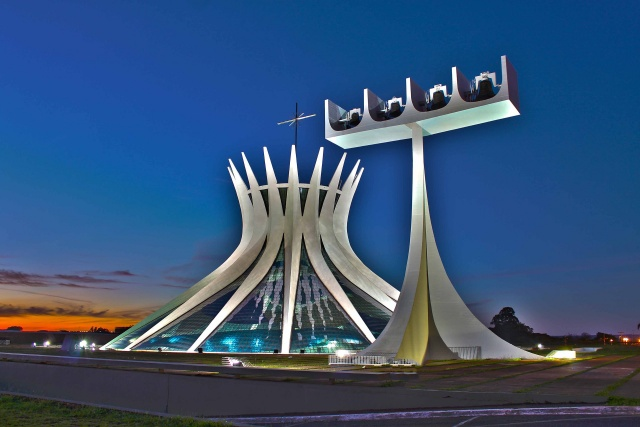
\includegraphics[width=0.8\textwidth]{figuras/figura-arquitetura}
	\caption{Arquitetura do sistema.}
	\label{figura-arquitetura}
\end{figure}

\vspace{0.5cm}

A arquitetura do sistema \emph{\imprimirtitulo} é baseada na Arquitetura em Camadas~\cite{tu2023layered}, adaptando a Arquitetura MVC~\cite{qureshi2014mvc}. Ela é composta por dois principais subsistemas, organizados em três camadas.
\begin{itemize}
	\item \textbf{Subsistema Controle Interno:} Responsável pelo gerenciamento interno do sistema, incluindo cadastro e manutenção de dados de funcionários, produtos, serviços e filiais.
	\item \textbf{Subsistema Atendimento Cliente:} Responsável pela interação com os clientes, abrangendo cadastro e login de clientes, agendamentos de serviços, histórico de atendimentos e registro de compras.
\end{itemize}
As camadas da arquitetura de cada subsistema são definidas como:
\begin{itemize}
	\item \textbf{Camada de Interface com o Usuário (CIU):} Responsável pela comunicação entre o usuário e o sistema, incluindo telas e controladores de interação.
	\item \textbf{Camada de Lógica de Negócio (CLN):} Implementa a lógica de aplicação e de domínio do problema. Aplica-se o padrão Camada de Serviço (Service Layer), separando a lógica de tarefas (CGT) da lógica de domínio (CDP).
	\item \textbf{Camada de Domínio do Problema (CDP):} Contém as classes que representam os conceitos e regras do domínio do problema.
	\item \textbf{Camada de Gerência de Dados (CGD):} Responsável pela persistência e recuperação de dados, seguindo o padrão Data Access Object (DAO).
\end{itemize}
A comunicação entre as camadas segue o padrão MVC, onde as páginas do front-end (CIU) chamam os adaptadores responsáveis pelas respostas via protocolo RESTful no back-end, acionando as classes controladoras (CIU), que interagem com as classes da camada de lógica de negócios (CLN) que, por sua vez, se comunicam com as classes do domínio do problema (CDP) e com as classes gerenciadoras de dados (CGD).

A comunicação entre CLN ocorre primeiro com a CGD ao invés de ocorrer com a CDP devido o mapeamento de entidades de domínio para modelos de tabelas no banco de dados, que é responsabilidade da CGD.
Contudo, a comunicação é feita através de interfaces, promovendo baixo acoplamento e facilitando a manutenção e evolução do sistema.

\vspace{0.5cm}

\vspace*{1.3cm}

\chapter{Projeto dos Componentes da Arquitetura}
\label{sec-componentes}
\vspace{-1cm}

Conforme mostrado na Figura~\ref{figura-arquitetura} ...

\vitor{A partir da arquitetura da Figura~\ref{figura-arquitetura}, descrever no parágrafo acima os subsistemas e as camadas de cada subsistema que serão apresentadas, ajustando as subseções abaixo conforme necessário e preenchendo-as com modelos e explicações textuais. Como exemplo, vide documentos de projeto do Marvin (caso em que há apenas 1 subsistema) e da Locadora de Carros do prof. Ricardo Falbo (caso em que há mais de um subsistema, como prevê este template).}


\section{Subsistema SS01}
\label{sec-componentes-ss01}

O subsistema SS01 ...

\vitor{Descrever o escopo do subsistema.}


\subsection{Camada de Negócio}
\label{sec-componentes-ss01-negocio}

\vitor{Apresentar os modelos e descrever no texto.}


\subsection{Camada de Apresentação}
\label{sec-componentes-ss01-apresentacao}

\vitor{Apresentar os modelos e descrever no texto.}


\subsection{Camada de Acesso a Dados}
\label{sec-componentes-ss01-dados}

\vitor{Apresentar os modelos e descrever no texto.}




\section{Subsistema SS02}
\label{sec-componentes-ss02}

O subsistema SS02 ...

\vitor{Descrever o escopo do subsistema.}


\subsection{Camada de Negócio}
\label{sec-componentes-ss02-negocio}

\vitor{Apresentar os modelos e descrever no texto.}


\subsection{Camada de Apresentação}
\label{sec-componentes-ss02-apresentacao}

\vitor{Apresentar os modelos e descrever no texto.}


\subsection{Camada de Acesso a Dados}
\label{sec-componentes-ss02-dados}

\vitor{Apresentar os modelos e descrever no texto.}
\endgroup



%%% Páginas finais do documento: bibliografia e anexos. %%%
% Finaliza a parte no bookmark do PDF para que se inicie o bookmark na raiz e adiciona espaço de parte no sumário.
\phantompart

% Marca o início dos elementos pós-textuais.
\postextual

% Referências bibliográficas
\bibliography{bibliografia}

% Índice remissivo.
\phantompart
\printindex

% Fim do documento.
\end{document}
